\chapter{実験2 -光沢感と明るさ感の関連性-}

    \section{目的}

        実験2では,実験1で使用した刺激と同じ色度を持つ単色パッチを用いて,H-K効果,すなわち色度による明るさ感の変化を用いて明るさを定量化する.
        実験1の色度による光沢感の変化と,実験2で計測される色度による明るさ感の変化を比較することで,色度による明るさ感の変化が光沢感に影響を及ぼした可能性について検討する.


    \section{実験方法}
        \subsection{実験環境,被験者}

            実験2で用いた装置と参加した被験者は,いずれも実験1と同一であった.

        \subsection{実験刺激}

            \begin{figure}[h]
                \centering
                
\includegraphics[width=14.0cm]{./img/ex2_stimuli2.png}
                \caption{実験刺激の例}
                \label{ex2_stimuli}
            \end{figure}

            \begin{figure}[h]
                \centering
                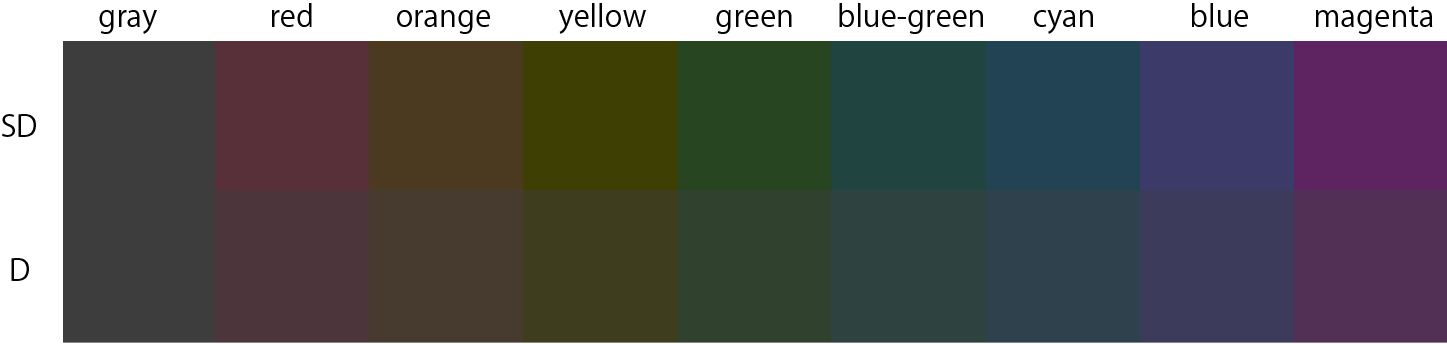
\includegraphics[width=14.0cm]{./img/ex2_stimuli_p.png}
                \caption{参照刺激として使われた色}
                \label{ex2_stimuli_set}
            \end{figure}
            \newpage

            実験2で使用する刺激と,参照刺激に使われた色を図\ref{ex2_stimuli}と図\ref{ex2_stimuli_set}に示す.
            参照刺激として使われた18種類の色度は,実験1で用いたDragon形状におけるSD条件,D条件のそれぞれの刺激の$XYZ$平均色に対応する.
            その輝度は,いずれの色度、彩色条件において5.80${\rm cd/m}^2$であった.
            [追記箇所: パッチの輝度]

        \subsection{実験手続き}

            \begin{figure}[h]
                \centering
                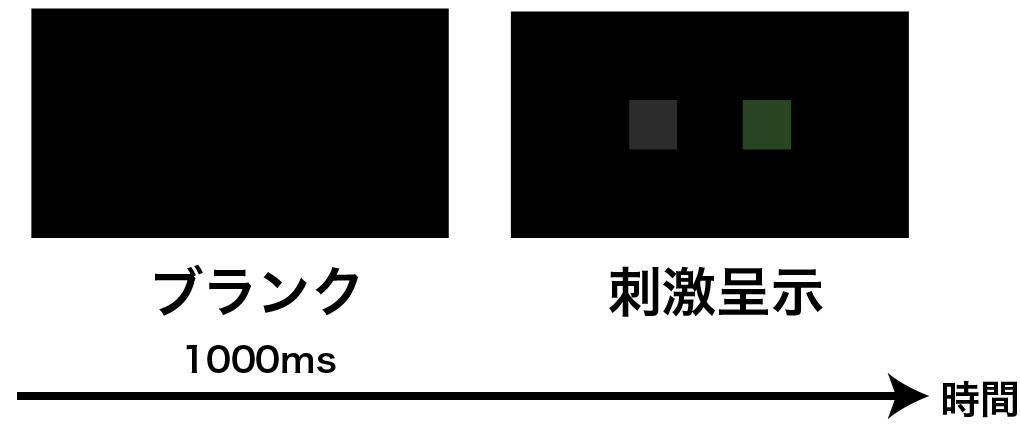
\includegraphics[width=10.0cm]{./img/ex2_procedure.png}
                \caption{1試行の流れ}
                \label{ex2_procedure}
            \end{figure}

            実験2では調整法によりカラーパッチの知覚的な明るさを計測する.
            実験2の1試行の流れを図\ref{ex2_procedure}に示す.
            各試行では,はじめに黒背景のみからなるブランク画面が1000msの間呈示された.
            次に,参照刺激であるカラーパッチとテスト刺激である無彩色パッチからなる刺激対が呈示された.
            この間に被験者はトラックボールを左右に回すことにより,無彩色パッチの輝度を調節でき,カラーパッチと同じ明るさに知覚されるようになるまで操作した.
            調整に満足したら,トラックボールマウスの右クリックを押すことその結果が記録され,そのままで次の試行のブランク画面へ移行した.
            なお,カラーパッチと無彩色パッチの左右位置は試行ごとにランダムに決定された.

            各セッションは2彩色条件$\times$色度9通り=18試行からなり,各被験者は全体で5セッションの実験を行った.
            各セッションの18試行で使われる参照刺激は全てランダムな順序で選ばれた.

    \section{実験結果}

        \subsection{H-K効果の大きさ}

            \begin{figure}[h]
                \centering
                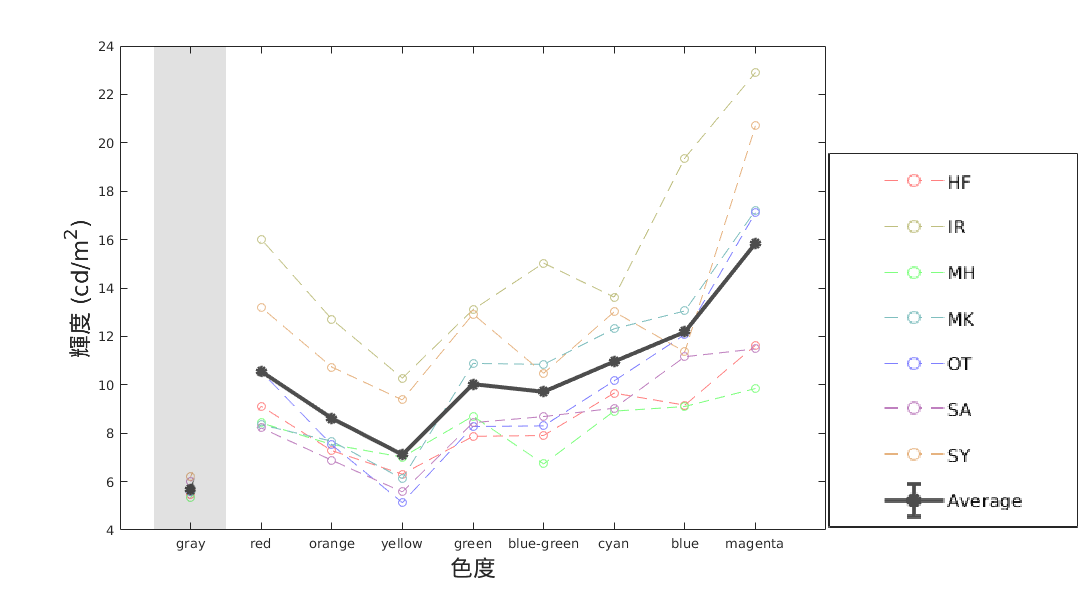
\includegraphics[width=14.0cm]{./img/ex2_res_SD_p.png}
                \caption{SD平均条件におけるテスト刺激の輝度}
                \label{ex2_SD}
            \end{figure}

            \begin{figure}[h]
                \centering
                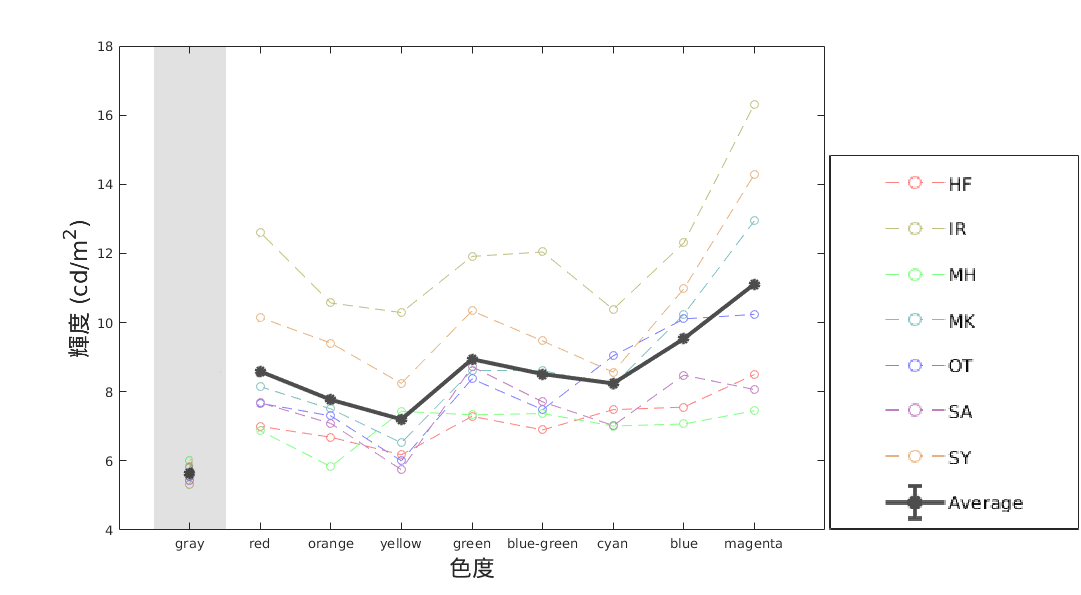
\includegraphics[width=14.0cm]{./img/ex2_res_D_p.png}
                \caption{D平均条件におけるテスト刺激の輝度}
                \label{ex2_D}
            \end{figure}


            図\ref{ex2_SD}がSD条件の結果,図\ref{ex2_D}がD条件の結果である.
            それぞれのグラフにおいて,横軸が刺激色,縦軸が被験者が調整したテスト刺激の輝度を示す.
            また,破線は被験者ごとの結果を表し,色が各被験者に対応している.
            黒実線は被験者間平均の結果を表す.
            どちらの条件においても,magentaの輝度が非常に高く,一方でgrayに次いでyellowの輝度が小さかった.

            [追記箇所: 統計]

            個人差に着目しても,SD条件,D条件共に色度に対する応答の傾向に大きな違いは見られなかった.
            また,有彩色のテスト刺激の輝度値は,全体的にD条件よりSD条件の方が大きかったが,これは刺激彩度が大きかったことによりH-K効果も強く出たものと考えられる.

            本実験により,実験1で用いた刺激の平均色に対するHK効果を定量化できた.
            次節では,この結果と実験1の結果から,光沢感と明るさの関連性を検証する.

    \newpage
        \subsection{実験1との関連性}

            \begin{figure}[h]
                \centering
                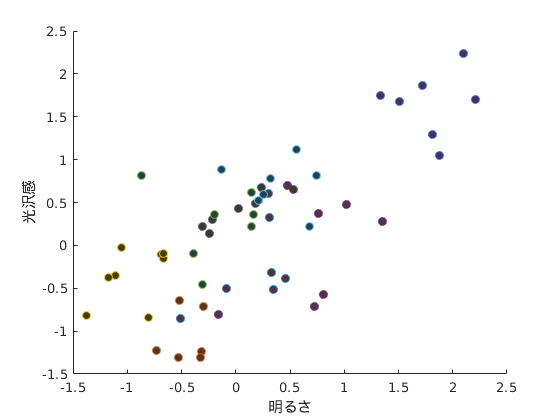
\includegraphics[width=11.0cm]{./img/ex3_DSD.png}
                \caption{Dragon形状のSD条件における散布図}
                \label{ex3_DSD}
            \end{figure}

            \begin{figure}[h]
                \centering
                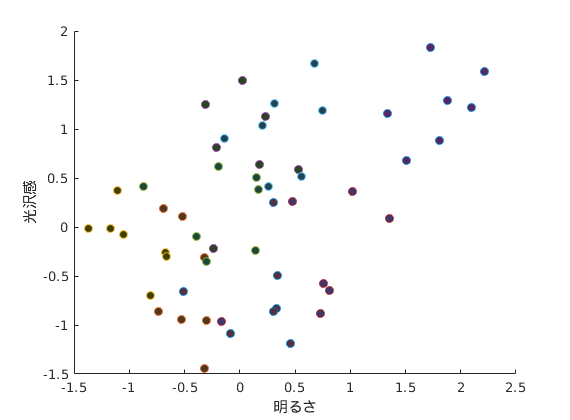
\includegraphics[width=11.0cm]{./img/ex3_BSD.png}
                \caption{Bunny形状のSD条件における散布図}
                \label{ex3_BSD}
            \end{figure}

            \newpage
            \begin{figure}[h]
                \centering
                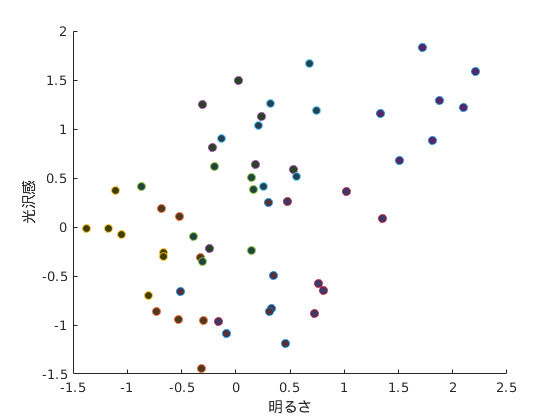
\includegraphics[width=11.0cm]{./img/ex3_DD.png}
                \caption{Dragon形状のD条件における散布図}
                \label{ex3_DD}
            \end{figure}

            \begin{figure}[h]
                \centering
                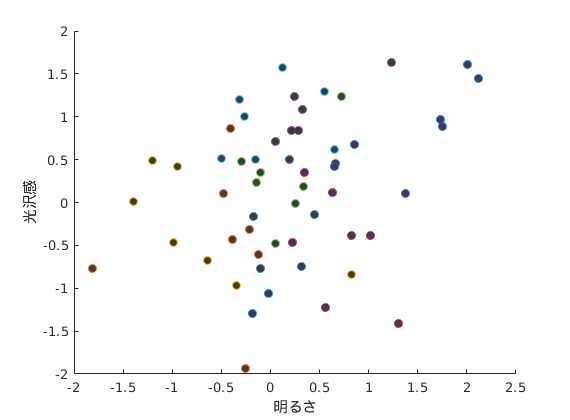
\includegraphics[width=11.0cm]{./img/ex3_BD.png}
                \caption{Bunny形状のD条件における散布図}
                \label{ex3_BD}
            \end{figure}

            \begin{table}[h]
                \centering
                \caption{各条件における実験1と実験2の結果の相関係数}
                \begin{tabular}{|l||c|c|} \hline
                                & SD       & D        \\ \hline \hline
                    Dragon      & 0.8828   & 0.8290   \\ \hline
                    Bunny       & 0.6490   & 0.5184   \\ \hline
                \end{tabular}
                \label{cc}
            \end{table}

            図\ref{ex3_DSD}から図\ref{ex3_BD}は,実験1と実験2のデータの両方に正規化を行い,物体形状と条件ごとに散布図にプロットしたものである.
            各点の色は実験で使われた9種類の色度からなり,横軸は明るさを,縦軸は光沢感を表す.
            また表\ref{cc}は各物体形状・着色条件における相関係数を表す.

            Dragon形状におけるSD条件,Dragon形状におけるD条件において比較的強い正の相関が見られたが,これに比べてBunny形状におけるSD条件,Bunny形状におけるD条件の相関係数は小さい値を示した.
            
            [追記箇所: 記述]
            さらに、知覚的な明るさに

        \subsection{考察}
        
            表\ref{cc}の結果は,H-K効果がもたらす知覚的な明るさは光沢感に寄与する要因の一つであるが,他の要因も寄与している可能性を示唆する.

            [追記箇所: 記述]

    \newpage